%!TEX root = ../MasterThesis.tex

\section{A partially centralized \gls{P2P} system proposal}
\label{sec:p2p_partially_centralized_system}

In the \gls{E-commerce} fraud scenario, which has been selected for this Master thesis in Section~\ref{sec:scope_thesis}, the issuer of a credit card is the participant, who initiates a collaborative session to investigate a malicious online transaction. Issuers are recognizing the active use (and maybe misuse) of a credit card in the online and the offline world first, and are also getting notifications about any suspicious activity from their fraud prevention systems. Due to these facts a valid design proposal for the \gls{E-commerce} fraud investigation system is based on a partially centralized \gls{P2P} communication network, in which the issuer of a credit card is taking over a leading position.

\subsection{Role of the issuer}
\label{subsec:p2p_partially_issuer_collecting}

In case a suspicious activity has been detected by the fraud prevention system of an issuer, one of their investigators will initiate a collaborative session with the relevant stakeholders that are selected based on the usage history of the credit card in question. To establish the \gls{P2P} communication session the investigator is creating a new \gls{WebRTC} communication session in the collaborative system, which has been implemented as a Web application. By doing so the investigator will receive a unique session ID that can be transmitted to merchants, \gls{PSP}s and \gls{LSP}s so that they can join in the collaborative system. As the investigator is just being aware of the \gls{PSP}s affected, they can invite them directly due to the existing business relationship between both parties. Based on the given credit card information the \gls{PSP}s can relate each payment authorization request to an order of an online merchant by referring to the payment authorization token. So the \gls{PSP}s will know the merchants that have to be involved in this \gls{E-commerce} fraud investigation, and can hand over contact information to invite them. Each online merchant can do likewise with the \gls{LSP} that has been used to handle the delivery of an order via the tracking number. \\

As soon as the relevant merchants, \gls{PSP}s and \gls{LSP}s have joined the \gls{P2P} communication session they will start sharing their information with the issuer. The information exchanged have been prepared as \gls{RDF} data sets by internal \gls{ETL} processes, and has been made available to the support staff of each stakeholder. In the process of information sharing the \gls{RDF} data sets of each stakeholder are replicated to the issuer, who will do the mapping and linking into a combined \gls{RDF} data store locally (as described in Section~\ref{sec:working_semantic_data}). This combination of the dispersed \gls{RDF} data sets will take place in a \gls{RDF} data store that the issuers have to setup and operate within their organization. Parts of this \gls{RDF} data store will take care of the reasoning over the merged \gls{RDF} data set to infer additional triple statements, as well as provide an internal \gls{SPARQL} endpoint to query the data store from the Web application as shown in Figure~\ref{fig:images_semweb_app}. \\

Thus, the major tasks will be done on the side of the issuers, who are coordinating and executing the \gls{E-commerce} fraud investigations as depicted in Figure~\ref{fig:images_p2p_centralized}.\@

\begin{figure}[H]
	\centering
		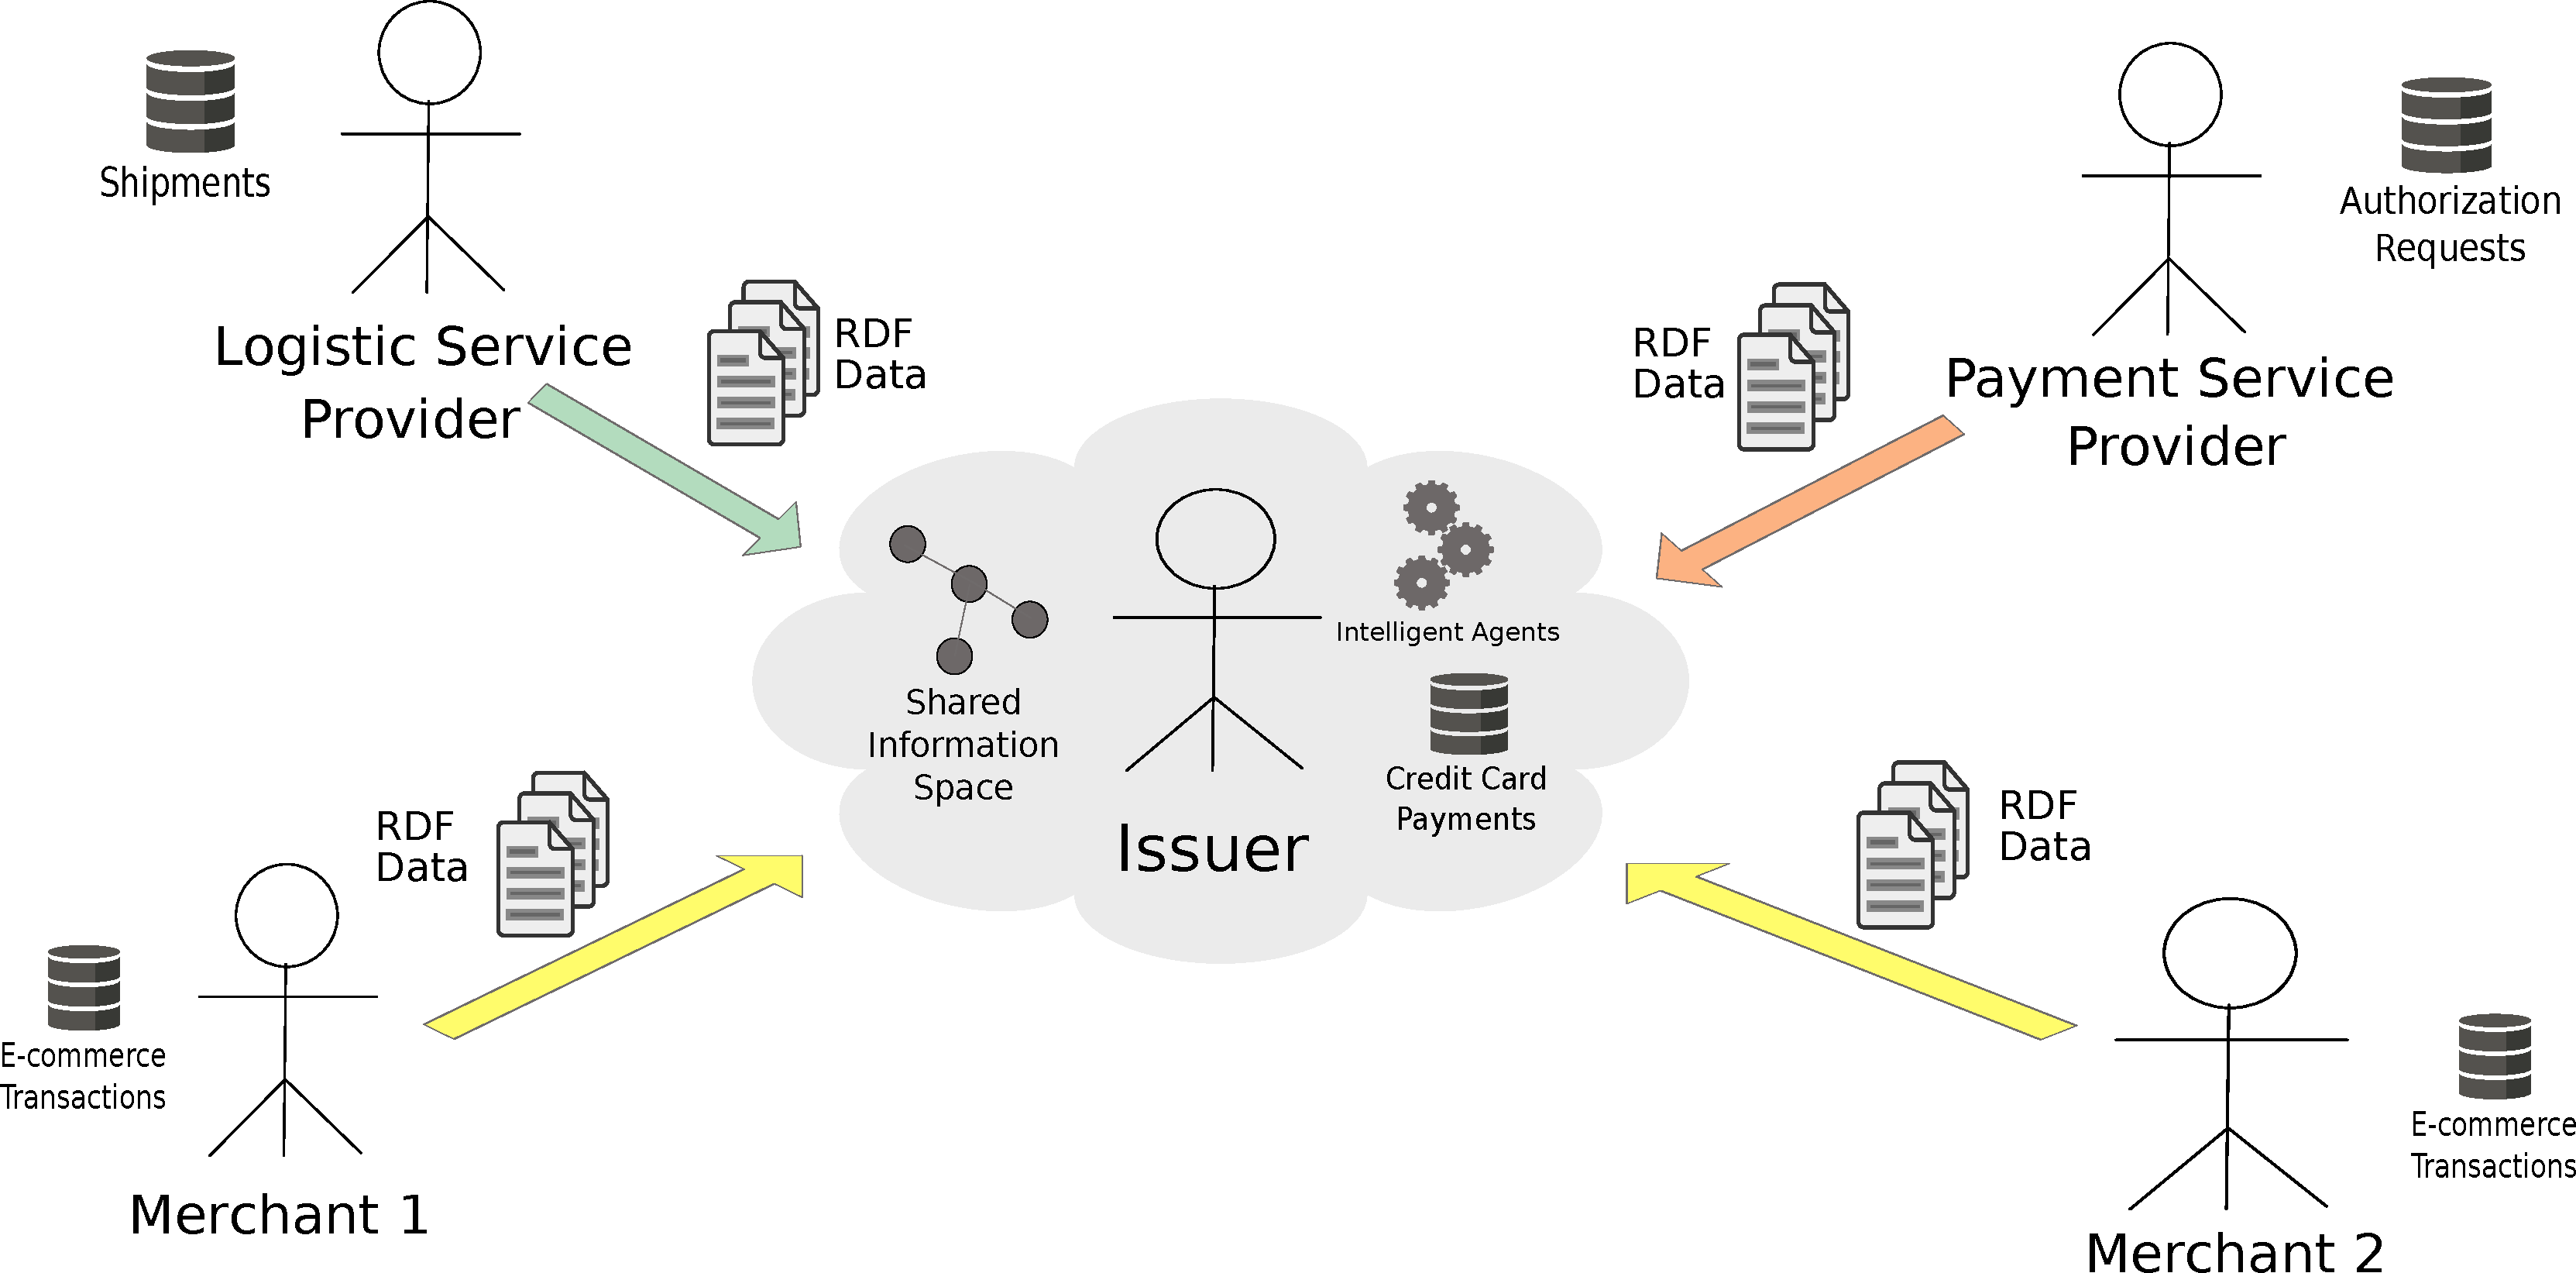
\includegraphics[width=0.9\columnwidth]{images/system_P2P_centralized.pdf}
	\caption{Collaborative system using a partially centralized \gls{P2P} architecture}
\label{fig:images_p2p_centralized}
\end{figure}


\subsection{Handling of privacy issues}
\label{subsec:p2p_partially_issuer_privacy}

One of the major concerns with the system architecture mentioned above is that the merchants, \gls{PSP}s and \gls{LSP}s have to hand over all of their relevant information to the issuer of a credit card for analyzing the \gls{E-commerce} activities of a consumer. This can raise severe privacy issues as an issuer will receive a lot of detailed order information from the other parties within this collaborative system. Issuers can not only use these information for validating the correctness of suspicious online transactions, but can also misuse them to build elaborate consumer profiles, which can directly influence the scoring of that consumer in the internal credit and risk rating systems of the issuers. \\

In addition to that online merchants will likely not provide to much detail information about their sales and offerings in such a collaborative system, because direct competitors might also be involved in the \gls{E-commerce} fraud investigation. By sharing parts of the business relevant information the merchants will raise the fear that their internal business processes, pricing structures as well as customer loyalty activities get more transparent to their competitors, which might lead to a stronger competition afterwards. \\

During the design of the collaborative system a valuation of the shared information has to take place, which classify each of them based on the criteria: \@

\begin{itemize}
	\item is the information really necessary to evalutate the \gls{E-commerce} transactions? Some of the order details from the merchants might not be required to analyze the transactions with the objective to find out an abnormal shopping behaviour.
	\item is the information worth protecting? Parts of the neccessary information are sensitive information and should be protected against misuse.
\end{itemize}

Special considerations have to be taken for mandatory \emph{and} sensitive information. In that case cryptographic algorithms such as hash functions (e.g.\ \gls{SHA-1}) can be used to anonymize the information. A hash function is working in one-direction only and generates a unique hash value based on its input parameter. This hash value is different as soon as the input changes only slightly, and due to the mathematical algorithms used for computing it a hash value can not be calculated back to the original input value of the hash function afterwards. \\

A valid use case for such a hashing of information is the e-mail address of a consumer. A plaintext e-mail address such as ``max.mustermann@web.de'' will always result in a \gls{SHA-1} value of ``8495914d9bd2c0c5d37ca351208a92e8b0ce2310'' regardless of the stakeholder, who has originally computed it. That is an additional benefit of the usage of hash functions, because they still allow the information from different stakeholders to be linked together based on their unique hash values. \\

Another approach to protect sensitive information is to consolidate them in a broader context --- a process called data generalization. An example for that would be the item categories, which can be split up into multiple hierarchical layers to narrowly define the affiliations of items to certain product groups. Instead of exchanging item descriptions with the complete set of categories they belong to, merchants can just share items and their top n categories to obfuscate detailed information about the products bought by a consumer. The same approach will also work for location based information, in which the shared information will not contain the exact geographic position from the original data set, but use an approximation to it by stating locations on a broader context (e.g.\ district, city or region) instead. \\

Based on these explanations the information, which is shared in the \gls{E-commerce} fraud investigation, can be classified into one of the following four quadrants, and should be handled as shown in Figure~\ref{fig:images_handle_privacy_concerns}. \@

\begin{figure}[H]
	\centering
		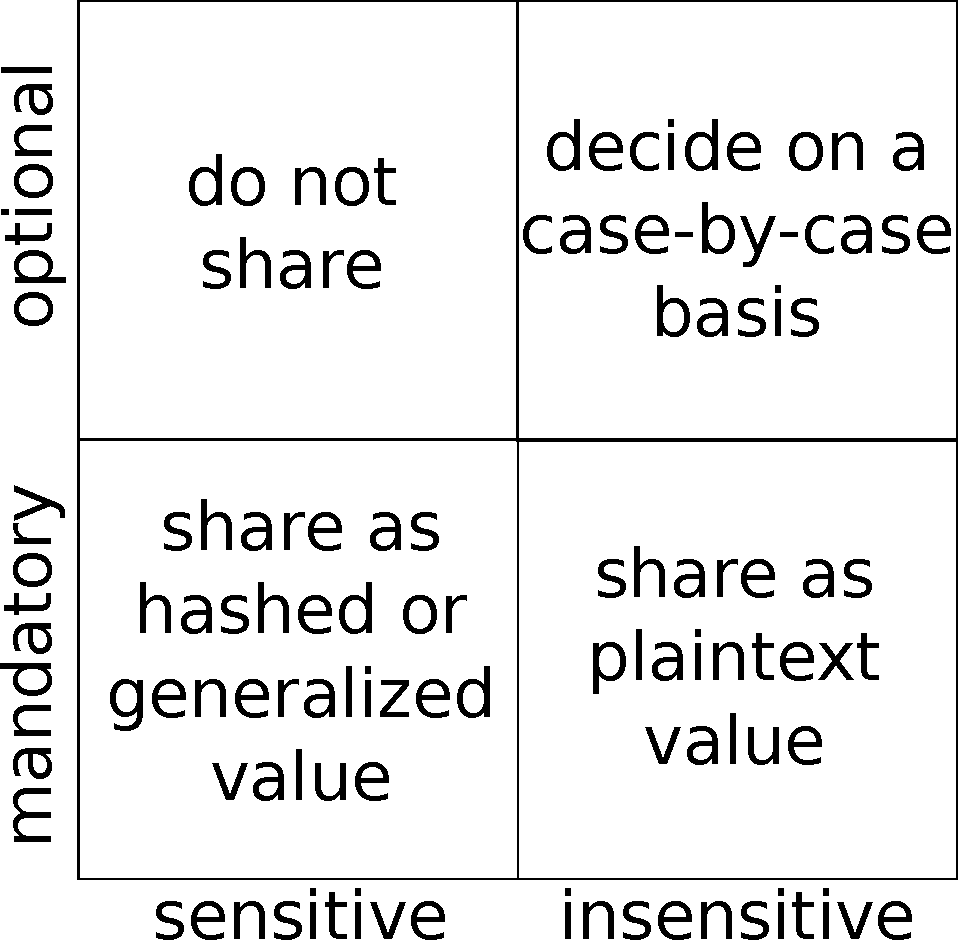
\includegraphics[width=0.5\columnwidth]{images/privacy_concerns.pdf}
	\caption{A possible classification of information in the collaborative system}
\label{fig:images_handle_privacy_concerns}
\end{figure}

% subsec p2p_partially_centralized_system

% section design_proposal (end)
